\documentclass{article}
\usepackage[utf8]{inputenc}
\usepackage{amsmath}
\usepackage{hyperref}
\usepackage{array}
\allowdisplaybreaks
\usepackage{graphicx}
\graphicspath{ {./images/} }

\title{Necklace}
\author{Maksymilian Demitraszek, Paweł Gmerek, Michał Kuliński}
\date{November 2021}

\begin{document}

\maketitle
\section{Abstract}
Necklace is a tiny, imperative, statically, strongly typed language with Elixir-like syntax.
Made for Group Project 1 \& 2 at Jagiellonian University


\section{Compiler architecture}
\subsection{Overview}
Necklace is a 2 phase compiler
\begin{itemize}
    \item Frontend - Lexer, Parser, Semantic checker
    \item Backend - code generation to LLVM
\end{itemize}
\begin{center}
    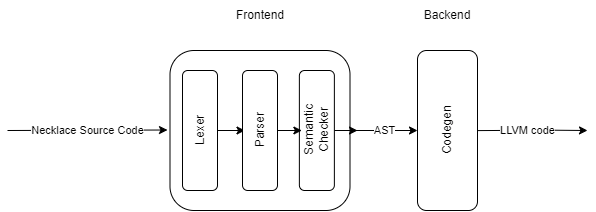
\includegraphics[scale=0.5]{compiler}
\end{center}
\subsection{Lexer}
The lexer is generated using the alex library for Haskell, which provides similar interface as lex. 

\subsection{Parser}
The parser is generated using the happy library for Haskell, which provides similar interface as yacc. 


\subsection{Semantic checker}
The language is statically and strongly checked. The compiler will perform a semantic analysis and throw errors if any of the types are not matching. 



\subsection{Code generation}
For the generation of LLVM IR representation we use the llvm-hs library which provides bindings simplifying the LLVM code generation



\section{Example syntax}
Every Necklacke program needs to have a main function that returns an integer.
\begin{verbatim}
function do_stuff(a: int, b: int) -> int do
    return 2 + 2;
end

function complex -> int do
    a: int;
    b: int;
    c: int;
    d: int;
    a = 1;
    b = 2;
    c = 3;
    d = a + b + c;
    return d;
end

function array_operations(a: *int, size: int) -> void do
    i: int;
    for (i = 0; i < size; i += 1) {
        (a + i)* +=1
    }
end


function main -> int do
    do_stuff(1, 2);
    return 0;
end
\end{verbatim}

\section{Tokens}
\subsubsection{Regular Expressions}
\begin{verbatim}
    @keywords = "(function|if|else|for|while|return|break|continue|->|do|end|alloc|free)"
    @varId = "[A-Za-z][A-Za-z0-9_]*"
    @int_lit = "([0-9])+" 
    @bool_lit = "true|false"
    @operator = "(\+|\-|\*|\/|%|<|>|>=|<=|==|!=|&&|\|\||!|=|>>|<<)"
    @comment = "~~.*"
    @special = "[\(\)\,\;\:\[\]\{\}]"
    @whitechar = "[\t\n\r\v\f\ ]"
    @type = int|bool
\end{verbatim}

\section{Grammar}
\begin{align*}
<start> &\longrightarrow \ <function>^* \\
<type> &\longrightarrow \ \textbf{bool} \ | \ \textbf{int} \ | \ \textbf{*} <type> \\
<return\_type> &\longrightarrow \ <type> \ | \ \textbf{void} \\
<function>  &\longrightarrow \\ 
    &| \ \textbf{function} <name> <arguments> \textbf{-\textgreater} <return\_type> \textbf{do} \ <function\_body> \ \textbf{end} \\
    &| \ \textbf{function} <name> \textbf{-\textgreater} <return\_type> \textbf{do} \ <function\_body> \ \textbf{end} 
    \\
    &| \ \textbf{function} <name> <arguments> \textbf{do} \ <function\_body> \ \textbf{end} \\
    &| \ \textbf{function} <name> <arguments> \textbf{do} \ <function\_body> \ \textbf{end} \\
<arguments> &\longrightarrow \ \textbf{(} <function\_args>\textbf{)} \\
<function\_args> &\longrightarrow \ <name> \textbf{:} <type> (\textbf{,} <name> \textbf{:} <type>)^* \\
<function\_body> &\longrightarrow \ <declaration>^* <statement>^+ \\
<body> &\longrightarrow \ <statement>^* \\
<statement> &\longrightarrow \ <function\_call>; \\
    &| \ <name> \textbf{=} <expression> \textbf{;}\\ 
    &| \ \textbf{if } <expr> \textbf{do} <body> \textbf{else} <body>  \ \textbf{end} \\
    &| \ \textbf{for (} <expr> \textbf{,} <expr> \textbf{,} <expr> \textbf{) do} <body> \textbf{end} \\ 
    &| \ \textbf{while} <expr> \textbf{do} <body> \textbf{end} \\
    &| \ \textbf{free} <expr>;
    &| \ \textbf{return} <expr> \textbf{;} \\
    &| \ \textbf{return;} \\
<declaration>  &\longrightarrow \ <name> \textbf{:} <type> \textbf{;} \\
<expression> &\longrightarrow \ <expression> <binary\_operator> <expression> \\
    &| \ <unary\_operator> <expression> \\
    &| \ ( <expression> ) \\
    &| \ <function\_call> \\
    &| \ <literal> \\
<unary\_operator> &\longrightarrow \ \textbf{*} \ | \ \textbf{-} \ | \ \textbf{!} \\
<binary\_operator> &\longrightarrow \ <arithmetic\_operator> \\ 
    &| \ <relational\_operator> \\
    &| \ <equality\_operator
    &| \ <conditional\_operator> \\
<arithmetic\_operator> &\longrightarrow \ \textbf{+} \
    | \ \textbf{-} \
    | \ \textbf{*} \
    | \ \textbf{/} \
    | \ \textbf{\%} \\
<relational\_operator> &\longrightarrow \ \textbf{\textless} \
    | \ \textbf{\textgreater} \
    | \ \textbf{\textless=} \
    | \ \textbf{\textgreater=} \\
<equality\_operator> &\longrightarrow \ \textbf{==} \ | \ \textbf{!=} \\
<conditional\_operator> &\longrightarrow \ \textbf{\&\&} \ | \ \textbf{$\mid\mid$} \\
<function\_call> &\longrightarrow \ <function\_name> ( <expr>^* ) \\
<function\_name> &\longrightarrow \ <name> \\
<literal> &\longrightarrow \ <int\_literal> \ | \ <bool\_literal> \\
<int\_literal> &\longrightarrow \ - <digit>^+|<digit>^+ \\
<bool\_literal> &\longrightarrow \ \textbf{true} \ | \ \textbf{false} \\
<identifier> &\longrightarrow \ <letter> \ | \ <identifier> <letter> \ | \ <identifier><digit> \\
\end{align*}
\subsection{Operators Precedence}
\begin{center}
\begin{tabular}{||c | c | c |  c|}
 \hline
 Priority & Category & Operator & Associativity\\
 \hline
 1 & Postfix  & $[$ $]$ & Left to right \\  
 \hline
 2 & Unary & $-$, $*$, $!$ & Right to left    \\
  \hline
 3 & Multiplicative & $*$, $/$, $\%$ & Left to Right    \\
 \hline
 4 & Additive & $+$, $-$ & Left to right \\ 
 \hline
 5 & Relational	& $<$, $>$, $<=$, $>=$ & Left to right\\
 \hline
 6 & Equality & $==$, $!=$ & Left to right \\
 \hline
 7 & Logical AND & $\&\&$ & Left to right \\
 \hline
 8 & Logical OR & $||$ & Left to right \\
 \hline
 9 & Assignment & $=$ & Right to left \\
 \hline
\end{tabular}
\end{center}
\section{Type system}
Necklace is a strongly typed language, so all type conversions have to be explicit.
\subsection{Base types}
\subsubsection{Boolean}
Declaration 
\begin{verbatim}
variable: bool;
\end{verbatim}
$$
\{true, false\}
$$
Corresponds to LLVMs i1 \url{https://releases.llvm.org/9.0.0/docs/LangRef.html#integer-type}
\subsubsection{Int}
Declaration 
\begin{verbatim}
variable: int;
\end{verbatim}

a 32 bit singed integer type \\
Corresponds to LLVMs i32 \url{https://releases.llvm.org/9.0.0/docs/LangRef.html#integer-type}
\subsubsection{Pointer}
\begin{verbatim}
variable: *<type>;
\end{verbatim}
Represents the location in memory of a variable
Corresponds to LLVMs pointer type \url{https://releases.llvm.org/9.0.0/docs/LangRef.html#pointer-type}
\subsubsection{Array}
Declaration 
\begin{verbatim}
variable: [<type>];
\end{verbatim}
Represents an array of variables of specified type
Corresponds to LLVMs array type \url{https://releases.llvm.org/9.0.0/docs/LangRef.html#array-type}

\subsection{Type inference}


\subsubsection{'-' unary operator}
$$
(+): int \longrightarrow int
$$

\subsubsection{'!' unary operator}
$$
(!): bool \longrightarrow bool
$$

\subsubsection{'*' unary operator}
$$
(*): pointer <type> \longrightarrow <type> 
$$

\subsubsection{'+' binary operator}
$$
(+): int \times int \longrightarrow int
$$

\subsubsection{'-' binary operator}
$$
(-): int \times int \longrightarrow int
$$

\subsubsection{'*' binary operator}
$$
(*): int \times int \longrightarrow int
$$

\subsubsection{'/' binary operator}
$$
(/): int \times int \longrightarrow int
$$

\subsubsection{'/' binary operator}
$$
(-): int \times int \longrightarrow int
$$
\subsubsection{'\%' binary operator}
$$
(\%): int \times int \longrightarrow int
$$
With behaviour defined as
$$
x\%y = r \ \ \ \ r = x - yk, x \in C
$$

\subsubsection{'toBool' conversion}
$$
toBool: int \longrightarrow bool
$$
With behaviour defined as
$$
toBool(x) =  \left\{ \begin{array}{ll}
false & x == 0  \\
true & otherwise \\
\end{array} \right.
$$

\subsubsection{'toInt' conversion}
$$
toInt: bool \longrightarrow int
$$
With behaviour defined as
$$
toInt(x) =  \left\{ \begin{array}{ll}
0 & x == false  \\
1 & x == true \\
\end{array} \right.
$$
\subsubsection{'$==$' binary operator}
$$
(==): int \times int \longrightarrow bool
$$
$$
(==): bool \times bool \longrightarrow bool
$$
\subsubsection{'$!=$' binary operator}
$$
(!=): int \times int \longrightarrow bool
$$
$$
(!=): bool \times bool \longrightarrow bool
$$

\subsubsection{'$<$' binary operator}
$$
(<): int \times int \longrightarrow bool
$$

\subsubsection{'$>$' binary operator}
$$
(>): int \times int \longrightarrow bool
$$
\subsubsection{'$<=$' binary operator}
$$
(<=): int \times int \longrightarrow bool
$$
\subsubsection{'$>=$' binary operator}
$$
(>=): int \times int \longrightarrow bool
$$
\subsubsection{'\&\&' binary operator}
$$
(\&\&): bool \times bool \longrightarrow bool
$$
\subsubsection{'$\mid\mid$' binary operator}
$$
(\mid\mid): bool \times bool \longrightarrow bool
$$
\subsubsection{'if' conditional operator}
$$
if \ bool \ do \ <block> \ end
$$
\subsubsection{'while' binary operator}
$$
while \ bool \ do \ <block> \ end
$$
\subsubsection{'for' binary operator}
$$
for \ <type> \ bool \ <type> \ do \ <block> \ end
$$

\section{Tests}
Necklace test suite includes unit tests for lexer and context sensitive analysis and integration tests for basic language functionalities.



\section{References}
\begin{enumerate}
    \item  Engineering a Compiler, by Keith D. Cooper & Linda Troczon
    \item MiT compilers course, decaf lang
\end{enumerate}

\end{document}